\documentclass[a4paper, 11pt]{article}

% packages
\usepackage[utf8]{inputenc}
\usepackage{amsmath}
\usepackage{amsfonts}
\usepackage{array}
\usepackage{booktabs}
\usepackage{chngcntr}
\usepackage{colortbl}
\usepackage{dcolumn}
\usepackage{float}
\usepackage{geometry}
\usepackage{graphicx}
\usepackage{hyperref}
\usepackage{multirow}
\usepackage{natbib}
\usepackage[normalem]{ulem}
\usepackage{ntheorem}
\usepackage{pdflscape}
\usepackage{rotating}
\usepackage{setspace}
\usepackage{subfigure}
\usepackage{tabularx}
\usepackage{threeparttable}
\usepackage[numbib, nottoc, notlot, notlof]{tocbibind}
\usepackage{wrapfig}
\usepackage{xcolor}

% page styling
\geometry{
  a4paper,
  left=1in,
  right=1in,
  bottom=1.2in,
  top=1.2in
}
\pagestyle{plain}
\pagenumbering{arabic}
\linespread{1.5}
\hypersetup{
  colorlinks,
  linkcolor={red!50!black},
  citecolor={blue!50!black},
  urlcolor={blue!80!black}
}
\theoremseparator{:}
\newtheorem{hyp}{Hypothesis}
\counterwithin*{hyp}{section}

\renewcommand{\thefootnote}{\fnsymbol{footnote}}

\title{
	% New title
	Insurance Tickets: Parties' Nomination Strategies in Japan's Mixed-Member Electoral System
	\footnotemark{}
	\footnotetext[1]{This paper was previously entitled ``Youth Underrepresentation and Parties' Nomination Strategy in Mixed-Member Electoral Systems" and presented at the 2024 Summer Meeting of the Japanese Society for Quantitative Political Science. The latest version of this paper is available at https://dxxsxsxkx.github.io.}
}


\author{
	Dai Sasaki
	\thanks{Master's Student, Graduate Schools for Law and Politics, The University of Tokyo. Email: daichansama12@g.ecc.u-tokyo.ac.jp}
}

\date{
	Prepared for the 2024 APSA Annual Meeting \\
	September 5 - 8, 2024
}

\begin{document}

\maketitle

\renewcommand{\thefootnote}{\arabic{footnote}}
\setcounter{footnote}{0}

\begin{abstract} 
While studies on parties' nomination strategies under proportional representation (PR) systems have accumulated, little is known about strategies in the PR tier embedded in mixed-member systems. This paper studies how parties allocate list positions to candidates under Japan's mixed-member systems, where candidates are allowed to run simulnaneously in the two tiers of the system (dual listing). Under dual listing, parties face a tradeoff between giving ``insurance tickets" to their exising members and nominating new candidates, where the former choice dominates the latter because of parties' post-election objectives. Analyzing the case of the Japanese House of Representatives election, I show that parties use dual listing to ensure the election of incumbents and senior members. These patterns are pronounced for the country's two majority-seeking parties and found even in elections after the dominant LDP had lost some of its senior members. The use of dual listing in mixed-member systems inhibits legislative turnover and could diminish representational advantages of PR systems. 
\end{abstract}

\newpage

\section{Introduction}

Scholars have long studied parties' nomination strategies with a focus on electoral systems, and many studies have analyzed nomination under proportional representation (PR) electoral systems \citep{buisseret_party_2022, crutzen_model_2020, dancygier_electoral_2014, hobolt_selection_2011, nemoto_localism_2013}. Under closed and flexible list PR systems, candidates' list position reflects parties' evaluation of them: this is primarily because their electoral prospects monotonically increase (or decrease) with their rank. Many studies have shown that placed higher on party lists are ``stronger" candidates, where candidates' ``strengths" refer to their cognitive ability \citep{buisseret_party_2022}, educational attainment \citep{buisseret_party_2022, cox_moral_2021}, previous electoral performances \citep{andre_party_2017, cox_moral_2021}, and so on. 

However, little is known about nomination strategies in the PR tier of mixed-member systems. A mixed-member system combines majoritarian and PR formulae within a single electoral system. There are broadly two types of mixed-member systems: one is called mixed-member majoritarian (MMM) or parallel system, which separately translates votes into seats in the majoritarian and PR tiers. The other one is called mixed-member proportional (MMP) system, where vote share in the PR tier determines the total number of seats a party obtains. Under such settings, it is not clear how parties formulate their candidate nomination strategies in the PR tier: on the one hand, they might give preferences to stronger candidates as they often do in pure PR systems. On the other hand, the simultaneuous use of two electoral formulae may induce interactions between the two tiers. Studies on mixed-member systems have pointed such ``contamination effects" (e.g., \citet{ferrara_mixed_2005}), and similar mechanisms might be observed regarding candidate nomination.  

This paper studies how parties allocate list positions to candidates under Japan's mixed-member systems. I claim that the nomination option of ``dual listing" in Japan's lower house election incentivizes parties to give second chances to their existing members, thereby limiting the number of new candidates they nominate. Japan's lower house election allows parties to nominate candidates simultaneously in a single-member district (SMD) and a PR block (``dual listing"). Dual-listed candidates have a second chance of election in the PR tier, even if they fail to win in the SMD tier. This institutional device allows parties to give ``insurance tickets" to their candidates. 

Under dual listing, parties face a tradeoff between giving “insurance tickets” to their exising members and nominating new candidates, where the former choice dominates the latter because of parties’ post-election objectives. Since parties have limited resources and cannot increase the number of nominees infinitely, they first estimate an obtainable number of seats and then allocate these winnable seats to candidates. In general, parties have incentives to prioritize senior politicians over junior members in candidate selection. Parties are not only vote-maximizing machines but also seek for post-election gains, such as policies, legislative activities, and ministerial posts. Experience matters in the pursuit of these goals: politicians accumulate resources over time and become more knowledgeable about policies, more effective in the legislature, and better qualified as party leadership and cabinet ministers. In the short run, parties may attempt to widen the breadth of their support by including new candidates in their lists. However, in the long run, government-seeking parties have incentives to ensure the election of more experienced members. 

Analyzing the nomination patterns of PR candidates in the Japanese lower house (House of Representatives; HoR) elections between 1996 and 2017, I show that parties use dual listing to ensure the election of incumbents and senior members using dual listing. Specifically, I find that dual-listed candidates, senior candidates, and incumbents tend to be placed higher on the list and that senior candidates and incumbents are more likely to be dual-listed. These patterns are particularly procounced for the country's two majority-seeking parties, namely the Liberal Democratic Party (LDP) and Democratic Party of Japan (DPJ) and its successor Constitutional Democratic Party (CDP). Smaller parties such as Komeito, LDP's long-term coalition partner, and Japanese Communist Party (JCP) do not rely on dual listing, although they do place senior candidates and incumbents higher on the list. In addition, the use of dual listing was prevalent even in elections after LDP had lost some of its senior members, namely the 2005 and 2012 elections. 

These findings on the nomination patterns under Japan's mixed-member system with dual listing have implications for studies on legislative turnover and minority representation. Given that the number of seats parties can obtain in an election is limited and predictable to some extent, parties are essentially solving an optimization problem where the constraint is the obtainable number of seats and the target functions are parties' various objectives. Parties have competing incentives to give second chances to existing members and to nominate new candidates, where the former dominates the latter due to the higher valence of senior politicians \citep{buisseret_party_2022}. Dual listing amplifies this first motivation and encourages parties to overprotect their exisiting candidates, which hinders the nomination and election of new candidates. 

In addition, the inherent representational advantages of PR systems could be diminished under mixed-member systems with dual listing. Scholars have argued that PR systems help augment the representation of minorities such as women and smaller ethinic groups (e.g., \citet{norris_electoral_2004}). As its name suggests, a PR system increases the proportionality between the number of votes and seats parties obtain. Under PR systems, even smaller parties that can only obtain a small number of votes, which often represent the interests of minorities, have a higher chance of winning seats. PR systems also induce parties to nominate candidates of a breadth of backgrounds, because they must appeal to a broader set of voters to gain more votes. However, as dual listing encourages parties to give second chances to their existing members, the incentives to diversify their lists weaken. Even though the level of minority representation could be somewhat maintained by the entry and survival of smaller parties, representation benefits of PR systems halve under mixed-member systems without proper institutional designs. 

This paper proceeds as follows. Section \ref{sec: the} discusses the theoretical backgrounds of the research, presents the main arguments, and formulate hypotheses. It first outlines Japan's mixed-member system with a focus on dual listing and then discusses how parties would render their nomination strategies where the two tiers are institutionally interacted. Section \ref{sec: emp} presents the data and empirical strategies. Section {sec: res} shows the results of the analysis. It presents aggregate-level and party-specific evidence, as well as election- and party-specific analysis. Section \ref{sec: dis} discusses the implication of the results, focusing on legislative turnover and representation. In addition, it provides conjectures about the relationship between Japan's electoral system and youth underrepresentation in the country. 

\section{Theory} \label{sec: the}

\subsection{Japan's Mixed-Member System}

In 1994, Japan undertook significant electoral reform by introducing a mixed-member electoral system that combines single-member districts (SMDs) with closed-list proportional representation (PR) blocks. This hybrid system was designed to integrate the strengths of both majoritarian and proportional representation systems, providing voters with two distinct votes. One vote is cast for a candidate in the SMD tier, where winners are determined by a first-past-the-post rule, a method that inherently favors the candidate with the most votes, even if they do not achieve an absolute majority. The other vote is cast for a party list in the PR tier, where seats are allocated based on the D'Hondt method—a highest averages method that distributes seats proportionally among parties according to their share of the vote. Within the PR tier, the distribution of seats to individual candidates is determined by their positions on the party list. The total number of seats a party secures is the cumulative result of its performance in both tiers. Japan's mixed-member system, therefore, is categorized as a "mixed-member majoritarian" (MMM) or "parallel system," distinct from "mixed-member proportional" (MMP) systems where a party's overall seat count is directly proportional to its PR vote share \citep{shugart_mixed-member_2003}.

A distinctive feature of Japan's MMM system is the provision for "dual listing," a mechanism that permits an interaction between the two electoral tiers by allowing candidates to be nominated simultaneously in both the SMD and PR tiers \citep{matland_determinants_2004, pekkanen2006electoral, reed2022}.\footnotemark{} \footnotetext{Similar dual listing practices are observed in other countries with mixed-member systems, such as Germany, New Zealand, Hungary, and Russia \citep{kono_dual_2020}} Under this system, political parties have the strategic option to nominate candidates in both tiers and assign them the same ranking on the PR list. After the election results are tallied, dual-listed candidates who win in their respective SMDs are removed from the PR list. Subsequently, the remaining dual-listed candidates with identical rankings are reordered according to the "best-loser" formula, which ranks them based on their performance in the SMD races. This practice of dual listing is not merely a theoretical option but a widespread and influential strategy in Japanese elections.

The prevalence of dual listing in Japan's electoral system is evident in its application over multiple election cycles. Data presented in Figure \ref{fig
} illustrates the significant share of PR winners who were dual-listed candidates in elections held between 1996 and 2017. Notably, since the 2000 election, a majority of legislators elected through the PR tier have been "zombies," a term used to describe dual-listed candidates who failed to win in their SMD contests but secured seats through their position on the PR list \citep{pekkanen2006electoral}. This trend has been particularly pronounced in the two largest political parties of the post-reform era: the Liberal Democratic Party (LDP), which has dominated Japanese politics for decades, and the Democratic Party of Japan (DPJ), later succeeded by the Constitutional Democratic Party (CDP). Both parties have consistently seen more than 50\% of their PR-elected legislators classified as zombies, indicating a strong reliance on dual listing to maintain legislative representation. In contrast, Komeito, the coalition partner of the LDP, has abstained from using dual listing since the early 2000s, marking a notable deviation from the prevailing trend. Overall, one can reasonably say that dual listing is a popular option in candidate nomination for the PR tier in post-reform Japanese politics. 

\footnotetext{Technically, candidates are reranked according to what is called ``close-loss rate". Let $i$ be a SMD-losing dual-listed candidate in the district $d$. Candidate $i$'s close loss rate, $\text{Loss}_{i}$, is calculated as 
  \[
    \text{Loss}_{i} = \frac{\text{Vote}_i}{\text{max}(\text{Vote}_d)}, 
  \]
\noindent where $\text{max}(\text{Vote}_d)$ denotes the largest number of votes obtained in the district $d$ (i.e., that of the winner). 
} 

\begin{figure}[!htbp]
	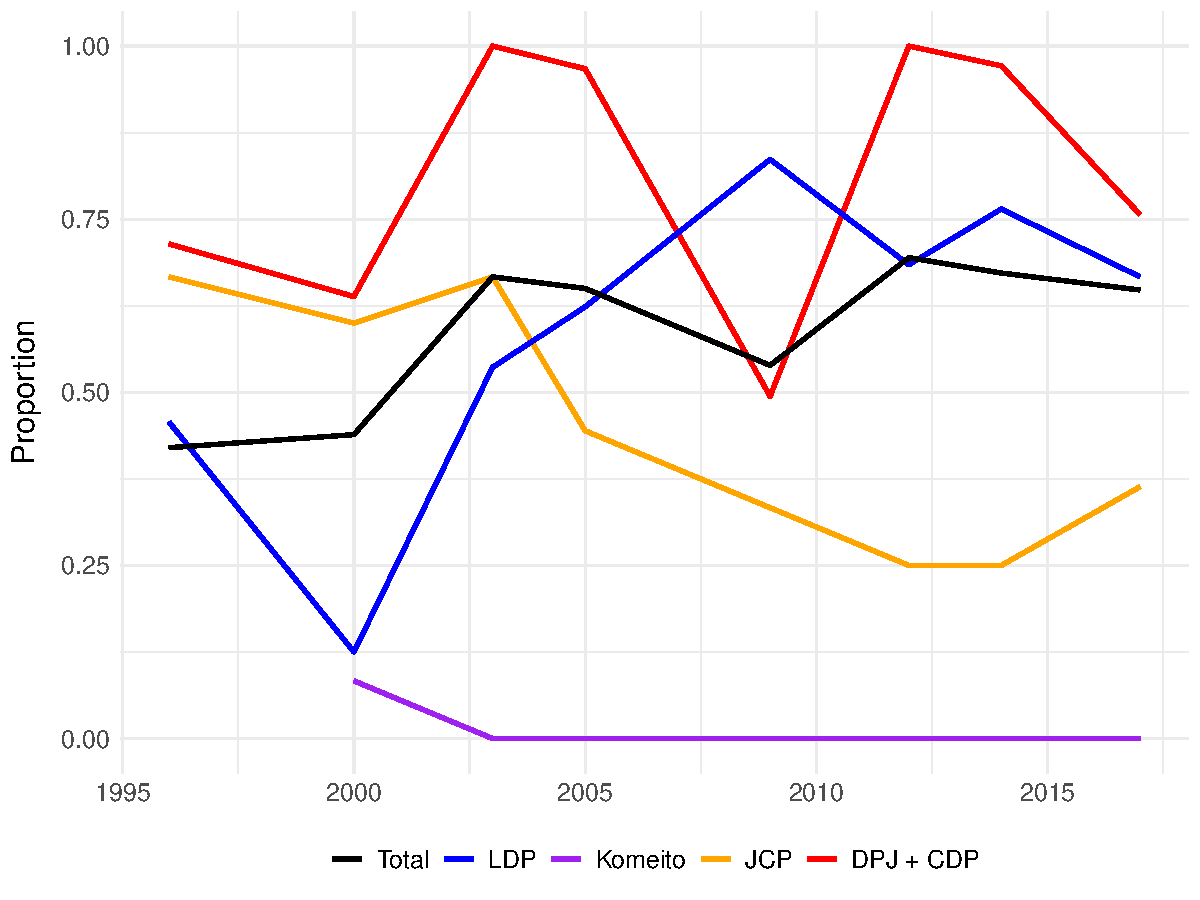
\includegraphics[width = 0.9\textwidth]{../figure/paper/dual_nomination.pdf}
	\caption{Share of Dual-Listed Candidates among PR Winners}
	\label{fig:dual}
\end{figure}


\subsection{Theoretical Expectations}

The existing body of research on candidate nomination within proportional representation (PR) systems is extensive (e.g., \citealt{buisseret_party_2022, cox_moral_2021}), yet there is limited understanding of whether analogous strategies and patterns are present within mixed-member electoral systems. Mixed-member systems are often characterized as offering “the best of both worlds” (\citealt{hirano_policy, shugart_mixed-member_2003}), effectively mitigating the extreme characteristics inherent to both pure majoritarian and pure proportional systems (\citealt{blais_electoral_1996, reynolds_electoral_2005, shugart_mixed-member_2003}). On the inter-party level, mixed-member systems are designed to maintain proportionality between vote shares and seat allocation, combining the majoritarian aspect, typically associated with two-party systems, with proportionality, which facilitates the emergence and persistence of smaller parties. For instance, mixed systems are posited to reduce the likelihood of parties without an absolute majority forming single-party governments, a common outcome in pure majoritarian systems. On the intra-party level, these systems are purported to simultaneously strengthen the relationship between candidates and their constituencies through the nominal tier while also enhancing party cohesion via the list tier.

A substantial body of literature has also addressed the phenomenon of "contamination" within mixed-member systems, referring to the spillover effects between electoral tiers (\citealt{cox_interaction_2002, ferrara_mixed_2005, herron_contamination_2001, nishikawa_mixed_2004, moser_mixed_2004}). These studies primarily focus on the implications of contamination for party systems, particularly concerning how the number of parties or candidates in mixed-member systems deviates from the theoretical predictions of Duverger's Law. Some scholars have examined party nomination strategies within mixed-member systems (\citealt{ferrara_going_2005}); however, their analyses predominantly address the inter-party dimension, specifically electoral coordination among parties, rather than the intra-party dimension, which is the focus of this paper.

Then, what are parties' candidate nomination strategies like in Japan's mixed-member system with dual listing? I argue that parties have incentives to prioritize senior candidates and incumbents in nomination and that dual listing encourages them to provide insurance tickets to these members. It is important for parties to maximize the number of votes and seats they obtain in the election, but as critical is to whom they allocate the seats obtained. Parties are not just vote-garnering devices active only during the election; they also have objectives at the post-election stage \citep{matakos_electoral_2024, strom1990behavioral, strom_policy_1999}. In this context, political parties face two competing incentives that create a strategic dilemma. On one hand, parties aim to secure the re-election of senior candidates who possess the experience and credibility to assume key governmental positions and internal party roles. Conversely, they must also facilitate the election of new candidates to ensure a pipeline of future senior members, thereby maintaining the party's long-term viability and renewal. Given that parties engage in electoral forecasting to estimate the feasible number of electable candidates, it can be argued that they are effectively solving a constrained optimization problem. The constraint in this case is the projected number of winnable seats, and the optimization involves balancing the retention of experienced members with the introduction of new political talent.

Consider a policy-oriented party with the primary objective of implementing its desired policies. For the party to achieve this goal, it is crucial that its members possess various resources: the ability to plan and legislate policies, knowledge of the legislative process, negotiation skills, coordination capabilities with the bureaucracy, and connections with key stakeholders. Politicians tend to acquire these resources as they accumulate experience in parliament, making it reasonable to assume a positive correlation between their years in office and the resources they possess. Consequently, incumbents, with their up-to-date knowledge and information, are generally better equipped than non-incumbents and are likely to be highly valued by the party.

If a party prioritizes members based on seniority and incumbency, this preference should be reflected in its nomination strategy. The practice of dual listing provides parties with an incentive to do so: they can offer "insurance tickets" to senior members and incumbents through this option. The value of this insurance varies; some candidates are placed at the top of the list, while others receive lower rankings, which they share with other dual-listed candidates. In a closed-list PR system, candidates with higher list rankings enjoy better electoral prospects.

Under dual listing, parties face a trade-off in nominating candidates for the PR tier: they can either offer second chances to candidates running in the SMD tier or nominate new candidates as pure-PR candidates. Given that the number of candidates a party can nominate is finite, this trade-off is significant. First, the party's resources, such as financial and logistical support, are limited. Second, parties typically refrain from nominating significantly more candidates than the number of seats they expect to win in the election. As a result, the number of newly nominated candidates decreases when parties dual-list existing members to enhance their electoral prospects.

Based on the above discussion, I argue that parties are inherently incentivized to prioritize senior candidates and incumbents in their nominations and that they are likely to offer these candidates second chances by dual-listing them. I propose the following five hypotheses for the aggregate-level analysis:

\begin{hyp}[H\ref{hyp:first}] \label{hyp:first}
Senior candidates are placed higher on the list. 
\end{hyp}

\begin{hyp}[H\ref{hyp:second}] \label{hyp:second}
Incumbents are placed higher on the list. 
\end{hyp}

\begin{hyp}[H\ref{hyp:third}] \label{hyp:third}
Senior candidates are more likely to be dual-listed; 
\end{hyp}

\begin{hyp}[H\ref{hyp:fourth}] \label{hyp:fourth}
Incumbents are more likely to be dual-listed; 
\end{hyp}

\begin{hyp}[H\ref{hyp:fifth}] \label{hyp:fifth}
Dual-listed candidates are placed higher on the lists. 
\end{hyp}

When examining individual political parties, it is plausible to hypothesize that the proposed Hypotheses 1-5 are broadly applicable across all parties. In the case of larger political parties, the potential to secure a substantial number of seats in each election, coupled with the possibility of forming a government, creates a strong incentive to ensure that candidates capable of assuming ministerial roles are successfully elected. Furthermore, these parties often possess a substantial number of members with extensive experience in various party roles, and there is frequently an established practice of distributing positions based on the number of electoral victories a candidate has achieved. These factors collectively amplify the incentives for larger parties to prioritize the provision of electoral insurance, particularly through dual listing, to senior and incumbent candidates.

Conversely, for smaller parties, while there is an inherent incentive to use the party list to increase the representation of younger legislators, it is also likely that these parties will employ dual listing as a strategy to secure the election of their core members. Given the high level of uncertainty surrounding the ability of smaller party core members to win in single-member districts, there is a strong incentive to place these individuals at the top of the list, thereby providing them with electoral insurance.

Moreover, the validity of Hypotheses 1 and 3 may be diminished in parties that have recently been ousted from power or have experienced internal strife. The incentive to provide insurance to senior candidates is partially driven by the need to allocate important governmental roles to these individuals. However, when a party loses its parliamentary majority and consequently falls from power, this need is substantially reduced. Similarly, in cases where a party enters an election amid unresolved internal factional disputes, the incentive to provide electoral insurance weakens. Under such circumstances, the dominant faction within the party may be inclined to marginalize members of rival factions.


\section{Data and Method} \label{sec: emp}

To test the hypotheses, I use the Japanese House of Representatives Elections Dataset (JHRED; \citet{reedsmith2018}). Specifically, I analyze the nomination patterns of candidates running in the PR tier of the post-reform general election between 1996 and 2017. This criterion leaves 6,935 candidates across eight elections (2000, 2003, 2005, 2009, 2012, 2014, 2017). Table \ref{tab:stats} in the appendix presents candidate-level summary statistics. 

For Hypotheses 1 and 2, I estimate logistic models that regress the dual listing dummy on the explanatory variable, the number of a candidate's past elections in the lower house elections, or the incumbency dummy, along with a set of covariates. I proxy candidates' seniority with the number of their past wins because politicians' seniority is measured by the number of terms they served in the same house \citep{pekkanen2006electoral}. The covariates include the female dummy, district magnitudes, and two-way fixed effects of election year and party. I control for candidates' gender because parties have incentives to give female candidates to appeal to a broader set of voters \citep{salmond2006proportional, chiru2017value}. I also account for block magnitudes, as the length of a list partially depends on the maximum number of candidates elected. Magnitudes vary across time and region: see Table \ref{tab:distM} in the appendix for details. Party fixed effects are supposed to account for different nomination patterns among parties. For example, \citet{fujimura2012position} finds different patterns for LDP and DPJ in allocating the parties' important positions. Given party-level variations in the candidate evaluation, it is reasonable to assume party-specific patterns of candidate nomination. For Hypotheses 3 and 4, I estimate negative binomial models that regress candidates' list rank on the explanatory variable and the same set of covariates. The application of negative binomial models is intended to account for the fact that the distribution of list rank is extremely right-skewed: see Figure \ref{fig:distRank} in the appendix for details.

\section{Result} \label{sec: res}

\subsection{Aggregate-Level Analysis}

Table \ref{tab:reg} presents the result of the regression analysis. All of the five hypotheses are supported after controlling for potential confounders. I find that the number of candidates' past elections and incumbency status are positively correlated with whether they are dual-listed in the PR tier. Candidates with more past elections and incumbents tend to be placed higher on the party list. These relationships hold regardless of candidates' gender, affiliated party, district magnitude, and election year. 


\begin{table}
\begin{center}
\begin{tabular}{l c c c c c c c c c c}
\hline
 & \multicolumn{4}{c}{List Rank} & \multicolumn{3}{c}{Dual Listing} & \multicolumn{3}{c}{Dual Listing (Tie)} \\
\cline{2-5} \cline{6-8} \cline{9-11}
 & Model 1 & Model 2 & Model 3 & Model 4 & Model 5 & Model 6 & Model 7 & Model 8 & Model 9 & Model 10 \\
\hline
Total Wins         & $-0.15^{***}$ &               &               & $-0.10^{***}$ & $0.16^{***}$ &              & $-0.00$      & $0.14^{***}$ &              & $0.00$        \\
                   & $(0.01)$      &               &               & $(0.02)$      & $(0.04)$     &              & $(0.02)$     & $(0.04)$     &              & $(0.02)$      \\
Incumbency         &               & $-1.02^{***}$ &               & $-0.74^{***}$ &              & $1.33^{***}$ & $1.33^{***}$ &              & $1.16^{***}$ & $1.13^{***}$  \\
                   &               & $(0.12)$      &               & $(0.11)$      &              & $(0.28)$     & $(0.28)$     &              & $(0.32)$     & $(0.31)$      \\
Dual Listing       &               &               & $-1.82^{***}$ & $-0.93^{***}$ &              &              &              &              &              &               \\
                   &               &               & $(0.25)$      & $(0.27)$      &              &              &              &              &              &               \\
Tie                &               &               &               & $-1.92^{*}$   &              &              &              &              &              &               \\
                   &               &               &               & $(0.86)$      &              &              &              &              &              &               \\
Female             &               &               &               & $-0.07$       &              &              & $-0.24^{*}$  &              &              & $-0.40^{***}$ \\
                   &               &               &               & $(0.04)$      &              &              & $(0.12)$     &              &              & $(0.11)$      \\
Block Magnitude    &               &               &               & $0.02^{***}$  &              &              & $0.04^{***}$ &              &              & $0.04^{***}$  \\
                   &               &               &               & $(0.01)$      &              &              & $(0.01)$     &              &              & $(0.01)$      \\
Total Wins x Tie   &               &               &               & $0.10^{***}$  &              &              &              &              &              &               \\
                   &               &               &               & $(0.02)$      &              &              &              &              &              &               \\
Tie x Incumbency   &               &               &               & $0.49^{**}$   &              &              &              &              &              &               \\
                   &               &               &               & $(0.18)$      &              &              &              &              &              &               \\
Tie x Dual Listing &               &               &               & $0.84$        &              &              &              &              &              &               \\
                   &               &               &               & $(0.91)$      &              &              &              &              &              &               \\
\hline
Year FE            & Yes           & Yes           & Yes           & Yes           & Yes          & Yes          & Yes          & Yes          & Yes          & Yes           \\
Party FE           & Yes           & Yes           & Yes           & Yes           & Yes          & Yes          & Yes          & Yes          & Yes          & Yes           \\
AIC                & $37167.39$    & $36446.03$    & $33098.42$    & $31652.57$    & $5886.23$    & $5697.89$    & $5629.09$    & $5949.29$    & $5803.79$    & $5729.36$     \\
Log Likelihood     & $-18536.69$   & $-18176.02$   & $-16502.21$   & $-15771.28$   & $-2897.12$   & $-2802.94$   & $-2765.54$   & $-2928.64$   & $-2855.90$   & $-2815.68$    \\
Num. obs.          & $7754$        & $7754$        & $7754$        & $7754$        & $7754$       & $7754$       & $7754$       & $7754$       & $7754$       & $7754$        \\
\hline
\multicolumn{11}{l}{\scriptsize{\item $^{***}p<0.001$; $^{**}p<0.01$; $^{*}p<0.05$. Standard errors clustered at the party level in parentheses.
\item Dependent variable: candidate $i$'s list rank (columns 1-4) dual listing status (columns 5-7), and whether the candidate has a tie on the list (columns 8-10).
\item Estimated models: negatige binomial (columns 1-4) and logit (columns 5-10).}}
\end{tabular}
\caption{Regression Results}
\label{tab:regression_results}
\end{center}
\end{table}


To illustrate these results within a specific context, I present several marginal effects plots. Using a hypothetical candidate profile, I modify the candidate's characteristics and examine the corresponding changes in the probability of being dual-listed and list rank. Specifically, the benchmark candidate is a male candidate affiliated with LDP, running in the Tokyo block in the 2012 election, which has the median block size of 17. Figure \ref{fig:dual} presents the predicted probabilities of the candidate being dual-listed, according to his incumbency status and the number of his previous wins in the election. Although the baselines are quite high, he is predicted to be significantly more likely to be dual-listed when he is a returning candidate or a candidate with past legislative experience. Specifically, the probability of dual listing is higher by more than ten percent when he is an incumbent. The relationship between seniority and dual-listing status is nonlinear, but he is about 10 percent more likely to be dual-listed when he has been elected five times compared to when he is a novice. 

\begin{figure}[!htbp]
	\caption{Dual Listing and Incumbency (Left); Seniority (Right)}
	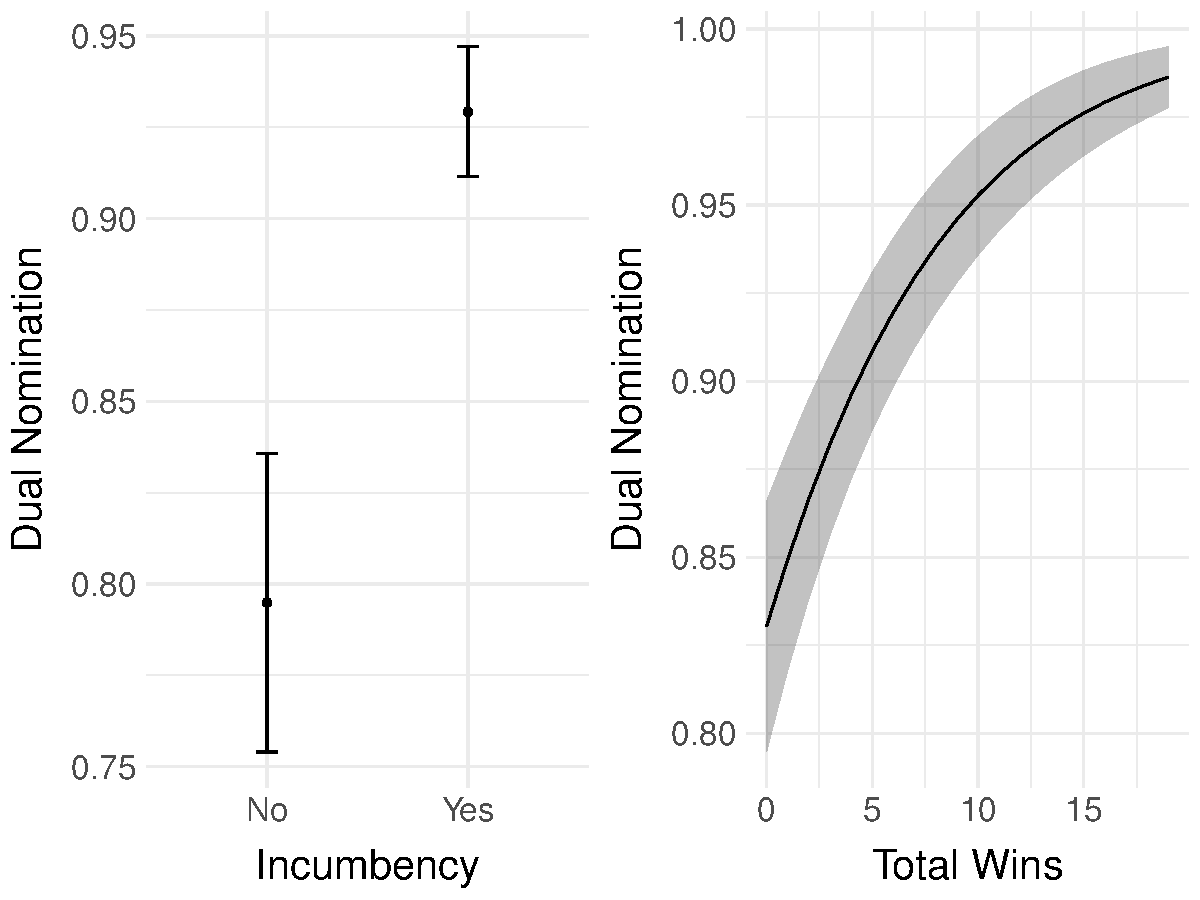
\includegraphics[width = 0.9\textwidth]{../figure/paper/h4_h5.pdf}
	\label{fig:dual}
\end{figure}

Figure \ref{fig:rank} presents the predicted list rank of the same hypothetical candidate. The three panels in the figure correspond to the relationships between rank and seniority (H3; top left), incumbency (H4; top right), and dual listing status (H5; bottom). Each of the three hypotheses is strongly supported: when the candidate is senior, an incumbent, or is dual listed, he is placed significantly higher on the party list. The differences are particularly pronounced for the cases of incumbency and dual listing status: he is predicted to be about five ranks above otherwise when he is an incumbent and more than ten ranks above when he is dual-listed. Overall, the two figures are illustrative of how parties give second chances to their senior members and incumbents by dual listing them or providing them with better positions on the party list. 

\begin{figure}[!thb]
	\caption{List Rank and Seniority (Top Left); Incumbency (Top Right); Dual Listing (Bottom)}
	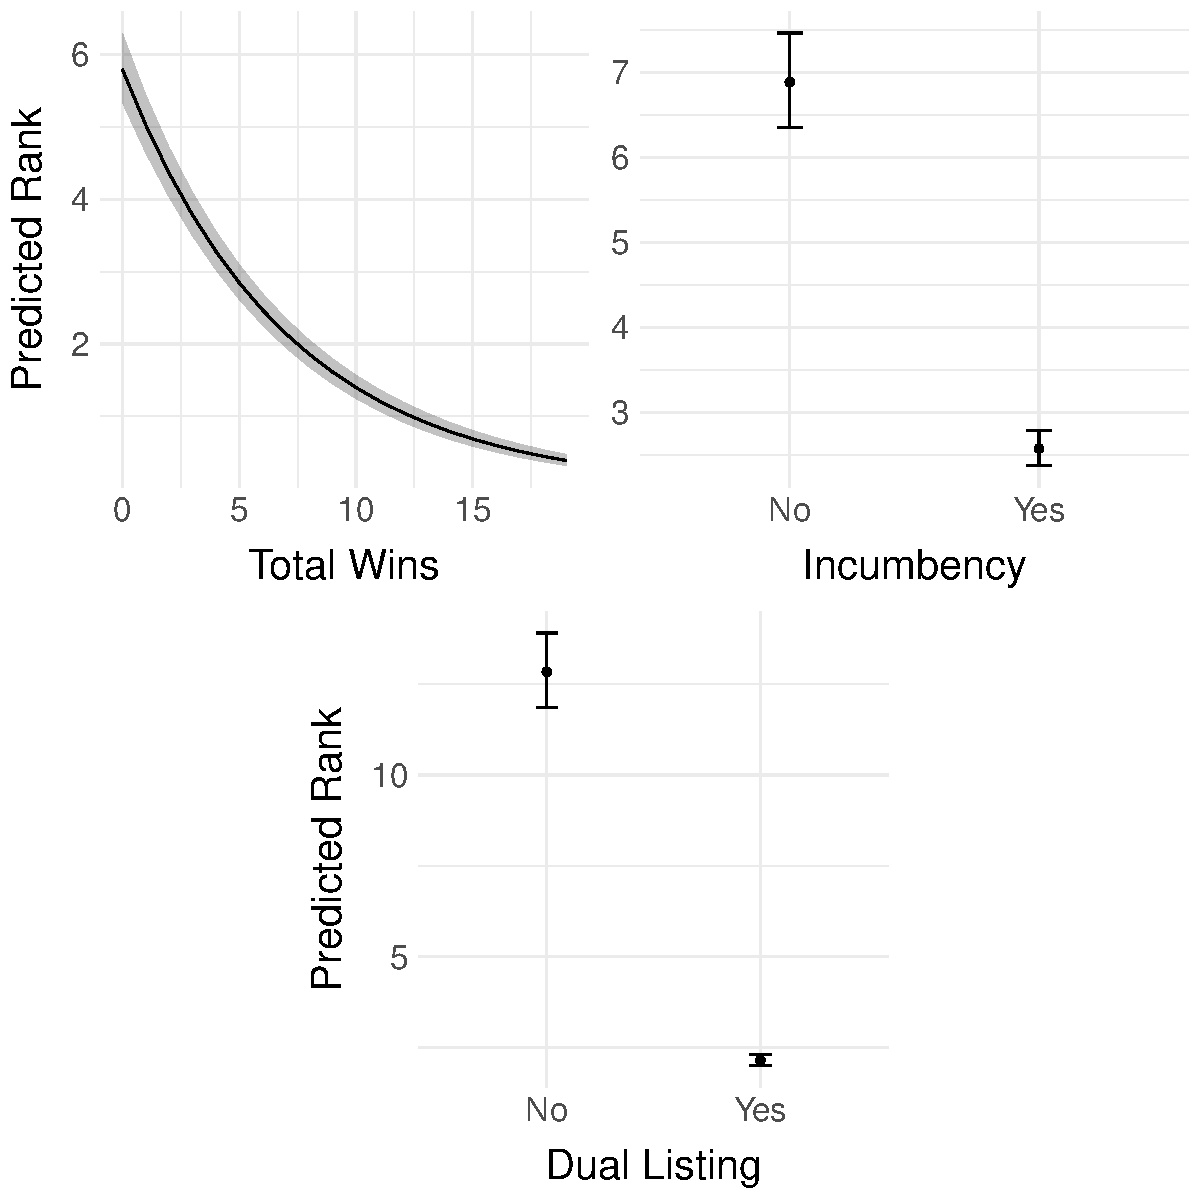
\includegraphics[width = 0.9\textwidth]{../figure/paper/h1_h2_h3.pdf}
	\label{fig:rank}
\end{figure}

\subsection{Party-Specific Analysis}

An examination of the validity of the five hypotheses requires a detailed analysis of the candidate nomination patterns across different political parties. In this analysis, I focus on two majority-seeking parties: the Liberal Democratic Party (LDP) and the Democratic Party of Japan (DPJ), including its successor, the Constitutional Democratic Party of Japan (CDP). These parties, characterized by their strategic efforts to achieve a parliamentary majority, offer a contrasting case study to the Japanese Communist Party (JCP), which, as a minor party, does not operate with majority-seeking objectives. \footnotemark{} By comparing these distinct political entities, I aim to elucidate how the hypotheses hold up under varying party goals and electoral strategies, particularly within the proportional representation (PR) tier of Japan's mixed-member electoral system.

\footnotetext{Table \ref{tab:regKomeito} in Appendix presents the nomination patterns of Komeito, a long-term coalition partner of the dominant LDP. Komeito's established policy of refraining from dual listing distinguishes it from other parties and warranted its exclusion from the primary analysis. The historical data further support this decision, as the occurrence of dual-listed candidates within the party has been minimal, rendering Hypotheses 1, 2, and 5 inapplicable. Nonetheless, the table indicates that incumbent and senior candidates receive preferential placement on the party list, suggesting that while dual candidacy is absent, internal party dynamics still influence the prioritization of candidates based on experience and tenure.}

Table \ref{tab:regLDP} shows the regression results for LDP candidates. A total of 2,589 candidates ran in the PR tier across eight general elections. All five hypotheses hold true: there is a positive significant relationship between both the number of prior electoral victories and the incumbent status of candidates with the likelihood of being dual-listed. Furthermore, these same variables exhibit a negative significant relationship with list positions, suggesting that senior and returning candidates are systematically allocated higher rankings on the PR list. This trend underscores the preferential treatment afforded to experienced and incumbent candidates within the nomination process, aligning with the theoretical expectations outlined in the hypotheses. Table \ref{tab:regDPJCDP} in Appendix exhibits the similar patterns of the candidates of DPJ and CDP. 


\begin{table}[!htbp]
\begin{center}
\scalebox{0.6}{
\begin{threeparttable}
\begin{tabular}{l D{.}{.}{5.5} D{.}{.}{5.5} D{.}{.}{5.5} D{.}{.}{5.5} D{.}{.}{5.5} D{.}{.}{5.5} D{.}{.}{5.5} D{.}{.}{5.5} D{.}{.}{5.5} D{.}{.}{5.5}}
\toprule
 & \multicolumn{4}{c}{List Rank} & \multicolumn{3}{c}{Dual Listing} & \multicolumn{3}{c}{Dual Listing (Tie)} \\
\cmidrule(lr){2-5} \cmidrule(lr){6-8} \cmidrule(lr){9-11}
 & \multicolumn{1}{c}{Model 1} & \multicolumn{1}{c}{Model 2} & \multicolumn{1}{c}{Model 3} & \multicolumn{1}{c}{Model 4} & \multicolumn{1}{c}{Model 5} & \multicolumn{1}{c}{Model 6} & \multicolumn{1}{c}{Model 7} & \multicolumn{1}{c}{Model 8} & \multicolumn{1}{c}{Model 9} & \multicolumn{1}{c}{Model 10} \\
\midrule
Total Wins         & -0.15^{***}             &                         &                         & -0.14^{***}             & 0.19^{***}              &                         & 0.01                    & 0.19^{***}              &                         & 0.02                    \\
                   & (0.01)                  &                         &                         & (0.01)                  & (0.02)                  &                         & (0.02)                  & (0.02)                  &                         & (0.02)                  \\
Incumbency         &                         & -1.26^{***}             &                         & -0.87^{***}             &                         & 1.64^{***}              & 1.65^{***}              &                         & 1.60^{***}              & 1.57^{***}              \\
                   &                         & (0.04)                  &                         & (0.07)                  &                         & (0.11)                  & (0.14)                  &                         & (0.11)                  & (0.14)                  \\
Dual Listing       &                         &                         & -2.00^{***}             & -1.52^{***}             &                         &                         &                         &                         &                         &                         \\
                   &                         &                         & (0.03)                  & (0.13)                  &                         &                         &                         &                         &                         &                         \\
Tie                &                         &                         &                         & -3.27^{***}             &                         &                         &                         &                         &                         &                         \\
                   &                         &                         &                         & (0.66)                  &                         &                         &                         &                         &                         &                         \\
Female             &                         &                         &                         & -0.17^{**}              &                         &                         & -0.58^{**}              &                         &                         & -0.70^{***}             \\
                   &                         &                         &                         & (0.05)                  &                         &                         & (0.18)                  &                         &                         & (0.17)                  \\
Block Magnitude    &                         &                         &                         & 0.01^{***}              &                         &                         & 0.05^{***}              &                         &                         & 0.05^{***}              \\
                   &                         &                         &                         & (0.00)                  &                         &                         & (0.01)                  &                         &                         & (0.01)                  \\
Total Wins x Tie   &                         &                         &                         & 0.14^{***}              &                         &                         &                         &                         &                         &                         \\
                   &                         &                         &                         & (0.01)                  &                         &                         &                         &                         &                         &                         \\
Tie x Incumbency   &                         &                         &                         & 0.71^{***}              &                         &                         &                         &                         &                         &                         \\
                   &                         &                         &                         & (0.08)                  &                         &                         &                         &                         &                         &                         \\
Tie x Dual Listing &                         &                         &                         & 2.51^{***}              &                         &                         &                         &                         &                         &                         \\
                   &                         &                         &                         & (0.67)                  &                         &                         &                         &                         &                         &                         \\
\midrule
Year FE            & \multicolumn{1}{c}{Yes} & \multicolumn{1}{c}{Yes} & \multicolumn{1}{c}{Yes} & \multicolumn{1}{c}{Yes} & \multicolumn{1}{c}{Yes} & \multicolumn{1}{c}{Yes} & \multicolumn{1}{c}{Yes} & \multicolumn{1}{c}{Yes} & \multicolumn{1}{c}{Yes} & \multicolumn{1}{c}{Yes} \\
Party FE           & \multicolumn{1}{c}{No}  & \multicolumn{1}{c}{No}  & \multicolumn{1}{c}{No}  & \multicolumn{1}{c}{No}  & \multicolumn{1}{c}{No}  & \multicolumn{1}{c}{No}  & \multicolumn{1}{c}{No}  & \multicolumn{1}{c}{No}  & \multicolumn{1}{c}{No}  & \multicolumn{1}{c}{No}  \\
AIC                & 16370.59                & 15871.58                & 14270.41                & 13692.05                & 2639.55                 & 2491.96                 & 2442.14                 & 2712.74                 & 2572.15                 & 2513.64                 \\
BIC                & 16436.29                & 15937.28                & 14336.11                & 13805.53                & 2699.27                 & 2551.68                 & 2519.78                 & 2772.47                 & 2631.88                 & 2591.28                 \\
Log Likelihood     & -8174.30                & -7924.79                & -7124.21                & -6827.03                & -1309.77                & -1235.98                & -1208.07                & -1346.37                & -1276.08                & -1243.82                \\
Deviance           & 2920.43                 & 2822.00                 & 2377.49                 & 2344.53                 & 2619.55                 & 2471.96                 & 2416.14                 & 2692.74                 & 2552.15                 & 2487.64                 \\
Num. obs.          & 2900                    & 2900                    & 2900                    & 2900                    & 2900                    & 2900                    & 2900                    & 2900                    & 2900                    & 2900                    \\
\bottomrule
\end{tabular}
\begin{tablenotes}[flushleft]
\scriptsize{\item $^{***}p<0.001$; $^{**}p<0.01$; $^{*}p<0.05$. Standard errors in parentheses.
\item Dependent variable: candidate $i$'s list rank (columns 1-4) dual listing status (columns 5-7), and whether the candidate has a tie on the list (columns 8-10).
\item Estimated models: negatige binomial (columns 1-4) and logit (columns 5-10).}
\end{tablenotes}
\end{threeparttable}
}
\caption{Regression Results for LDP Candidates}
\label{tab:ldp}
\end{center}
\end{table}


Table \ref{tab:regJCP} presents the results for JCP. There has been 426 candidates running in the PR tier of the post-reform general elections. For JCP, only Hypotheses 3 and 4 are applicable: there are negative significant relationships between list rank and each of the number of prior elections and the incumbency status. However, I find no significant relationships regarding dual listing status, although JCP did use the dual-listing option in each of the eight elections as Figure \ref{fig:dual} shows. 


\begin{table}[!htbp]
\begin{center}
\scalebox{0.7}{
\begin{threeparttable}
\begin{tabular}{l D{.}{.}{4.5} D{.}{.}{4.5} D{.}{.}{4.3} D{.}{.}{4.5} D{.}{.}{4.3} D{.}{.}{4.3} D{.}{.}{4.5} D{.}{.}{3.3} D{.}{.}{5.3} D{.}{.}{5.5}}
\toprule
 & \multicolumn{4}{c}{List Rank} & \multicolumn{3}{c}{Dual Listing} & \multicolumn{3}{c}{Dual Listing (Tie)} \\
\cmidrule(lr){2-5} \cmidrule(lr){6-8} \cmidrule(lr){9-11}
 & \multicolumn{1}{c}{Model 1} & \multicolumn{1}{c}{Model 2} & \multicolumn{1}{c}{Model 3} & \multicolumn{1}{c}{Model 4} & \multicolumn{1}{c}{Model 5} & \multicolumn{1}{c}{Model 6} & \multicolumn{1}{c}{Model 7} & \multicolumn{1}{c}{Model 8} & \multicolumn{1}{c}{Model 9} & \multicolumn{1}{c}{Model 10} \\
\midrule
Total Wins       & -0.22^{***}             &                         &                         & -0.10^{***}             & -0.03                   &                         & -0.04                   & -2.19^{*}               &                         & -1.40                   \\
                 & (0.02)                  &                         &                         & (0.03)                  & (0.05)                  &                         & (0.08)                  & (0.98)                  &                         & (1.13)                  \\
Incumbency       &                         & -0.95^{***}             &                         & -0.72^{***}             &                         & -0.12                   & -0.17                   &                         & -19.85                  & -17.22                  \\
                 &                         & (0.08)                  &                         & (0.11)                  &                         & (0.23)                  & (0.34)                  &                         & (2367.75)               & (2043.44)               \\
Dual Listing     &                         &                         & 0.07                    & -0.06                   &                         &                         &                         &                         &                         &                         \\
                 &                         &                         & (0.06)                  & (0.06)                  &                         &                         &                         &                         &                         &                         \\
Tie              &                         &                         &                         & -0.03                   &                         &                         &                         &                         &                         &                         \\
                 &                         &                         &                         & (0.11)                  &                         &                         &                         &                         &                         &                         \\
Female           &                         &                         &                         & 0.04                    &                         &                         & -0.12                   &                         &                         & -0.99^{*}               \\
                 &                         &                         &                         & (0.05)                  &                         &                         & (0.21)                  &                         &                         & (0.46)                  \\
Block Magnitude  &                         &                         &                         & 0.05^{***}              &                         &                         & 0.07^{***}              &                         &                         & 0.13^{***}              \\
                 &                         &                         &                         & (0.00)                  &                         &                         & (0.01)                  &                         &                         & (0.04)                  \\
Total Wins x Tie &                         &                         &                         & 0.29                    &                         &                         &                         &                         &                         &                         \\
                 &                         &                         &                         & (0.51)                  &                         &                         &                         &                         &                         &                         \\
\midrule
Year FE          & \multicolumn{1}{c}{Yes} & \multicolumn{1}{c}{Yes} & \multicolumn{1}{c}{Yes} & \multicolumn{1}{c}{Yes} & \multicolumn{1}{c}{Yes} & \multicolumn{1}{c}{Yes} & \multicolumn{1}{c}{Yes} & \multicolumn{1}{c}{Yes} & \multicolumn{1}{c}{Yes} & \multicolumn{1}{c}{Yes} \\
Party FE         & \multicolumn{1}{c}{No}  & \multicolumn{1}{c}{No}  & \multicolumn{1}{c}{No}  & \multicolumn{1}{c}{No}  & \multicolumn{1}{c}{No}  & \multicolumn{1}{c}{No}  & \multicolumn{1}{c}{No}  & \multicolumn{1}{c}{No}  & \multicolumn{1}{c}{No}  & \multicolumn{1}{c}{No}  \\
AIC              & 1775.10                 & 1750.64                 & 1897.57                 & 1568.00                 & 628.43                  & 628.60                  & 610.54                  & 178.03                  & 180.35                  & 162.47                  \\
BIC              & 1820.69                 & 1796.23                 & 1943.16                 & 1638.45                 & 669.87                  & 670.04                  & 664.42                  & 219.48                  & 221.79                  & 216.34                  \\
Log Likelihood   & -876.55                 & -864.32                 & -937.78                 & -767.00                 & -304.21                 & -304.30                 & -292.27                 & -79.02                  & -80.18                  & -68.23                  \\
Deviance         & 385.60                  & 372.88                  & 423.51                  & 191.69                  & 608.43                  & 608.60                  & 584.54                  & 158.03                  & 160.35                  & 136.47                  \\
Num. obs.        & 466                     & 466                     & 466                     & 466                     & 466                     & 466                     & 466                     & 466                     & 466                     & 466                     \\
\bottomrule
\end{tabular}
\begin{tablenotes}[flushleft]
\scriptsize{\item $^{***}p<0.001$; $^{**}p<0.01$; $^{*}p<0.05$. Standard errors in parentheses.
\item Dependent variable: candidate $i$'s list rank (columns 1-4) dual listing status (columns 5-7), and whether the candidate has a tie on the list (columns 8-10).
\item Estimated models: negatige binomial (columns 1-4) and logit (columns 5-10).}
\end{tablenotes}
\end{threeparttable}
}
\caption{Regression Results for JCP Candidates}
\label{tab:jcp}
\end{center}
\end{table}


In summary, the preferential treatment of incumbent and senior candidates through dual candidacy is not a universal strategy across all political parties. Among the three parties analyzed, LDP and DPJ / CDP exhibit a higher propensity to employ dual candidacy for these categories of candidates. In contrast, JCP does not consistently apply this approach. Nevertheless, even within the JCP, there exists a discernible tendency to grant preferential treatment to incumbent and senior candidates, particularly in terms of their placement on the party list. This suggests that while parties are generally incentivized to prioritize established candidates, the specific mechanisms they use to confer these advantages vary significantly depending across parties. 

\subsection{Election- / Party-Specific Analysis}

The subsequent analysis investigates the applicability of the proposed hypotheses within the context of a specific political party during a particular election. It is hypothesized that the validity of Hypotheses 1 and 3 may be diminished in cases where the party in question has either recently transitioned out of power or has been embroiled in internal strife. To explore this, I focus on LDP in the context of the Japanese House of Representatives elections held in 2005 and 2012.

The House of Representatives election in September 2005, widely known as the "Yusei Senkyo (Postal Election)," was precipitated by the dissolution of the legislature following the rejection of the Postal Privatization Bill in the House of Councillors the preceding month. For Prime Minister Junichiro Koizumi, the bill represented a central policy initiative that he had championed even before his tenure as Prime Minister \citep{uchiyama_2007}. However, the legislative process was marked by significant resistance from within the party. In an unprecedented move, Koizumi circumvented the conventional pre-legislative scrutiny within the party to bring the bill directly before the plenary session of the House of Representatives.\footnotemark{} Although the bill narrowly passed in the House of Representatives, it was ultimately rejected by the House of Councillors. Throughout this process, a total of 51 LDP members in the House of Representatives and 22 members in the House of Councillors dissented by voting against the bill or absenting from the session. 

\footnotetext{In the LDP government, it is standard procedure for bills proposed by the cabinet to undergo preliminary review by the LDP's Soumukai (General Council) before being presented to the Diet. Party regulations stipulate that decisions within the General Council are typically made by a majority vote. However, the principle of achieving unanimous agreement is commonly upheld as a procedural norm. The Postal Privatization Bill, which was subject to this review process, advanced through the General Council by securing a majority vote, despite the usual emphasis on achieving consensus.}

Following the rejection of the bill, Koizumi dissolved the House of Representatives and called a general election. During this election, he revoked the official endorsement of the members who had rebelled during the bill's vote and placed other officially endorsed candidates in their constituencies. The displaced members either contested the election as independents or established new political parties to do so. The Liberal Democratic Party (LDP) secured a landslide victory in this election, followed by the swift passage of the once-denied Postal Privatization Bill through both chambers of the Diet shortly thereafter. This turnover of members might have resulted in changed to the candidate nomination patterns in the PR tier. 

In the 2009 general election, the LDP suffered a significant defeat, losing its majority and being ousted from power.  The DPJ won 308 of the 480 available seats, while the LDP’s representation plummeted from 300 seats before the election to just 119. However, in the 2012 election, the LDP staged a comeback, winning 294 seats and regaining power. The turnover in members might have also led to changes in the candidate nomination patterns. 

Table \ref{tab:regLDP2005_2012} presents the results of the analysis of the LDP’s candidate nomination patterns in the 2005 and 2012 elections. The hypotheses were not rejected: in both the 2005 and 2012 cases, legislators with longer tenure were more likely to be dual-listed and positioned higher on the list. The magnitude of the coefficients was consistent with the aggregate case. In neither of these elections did the LDP deprioritize senior candidates; thus, it can be argued that the party's policy of prioritizing incumbents and senior legislators remained consistent, even in the face of internal conflicts and changes in government.


\begin{table}
\begin{center}
\begin{tabular}{l c c c c c}
\hline
 & \multicolumn{3}{c}{2005} & \multicolumn{2}{c}{2012} \\
\cline{2-4} \cline{5-6}
 & List Rank & Dual Listing & Tie & List Rank & Dual Listing \\
\hline
Total Wins         & $-0.01$       & $0.03$       & $0.06$       & $0.02$        & $0.61^{*}$   \\
                   & $(0.02)$      & $(0.09)$     & $(0.08)$     & $(0.04)$      & $(0.25)$     \\
Incumbency         & $-2.03^{***}$ & $1.76^{***}$ & $1.47^{***}$ & $-0.23$       & $1.48$       \\
                   & $(0.16)$      & $(0.46)$     & $(0.42)$     & $(0.28)$      & $(1.21)$     \\
Dual Listing       & $-1.77^{***}$ &              &              & $-3.41^{***}$ &              \\
                   & $(0.17)$      &              &              & $(0.09)$      &              \\
Tie                & $-3.26^{**}$  &              &              &               &              \\
                   & $(1.01)$      &              &              &               &              \\
Female             & $-0.56^{***}$ & $0.52$       & $-0.31$      & $-0.06$       & $0.57$       \\
                   & $(0.10)$      & $(0.59)$     & $(0.48)$     & $(0.12)$      & $(0.69)$     \\
Block Magnitude    & $0.04^{***}$  & $0.04$       & $0.05^{*}$   & $0.04^{***}$  & $0.10^{***}$ \\
                   & $(0.00)$      & $(0.02)$     & $(0.02)$     & $(0.00)$      & $(0.03)$     \\
Total Wins x Tie   & $0.01$        &              &              &               &              \\
                   & $(0.02)$      &              &              &               &              \\
Tie x Incumbency   & $2.00^{***}$  &              &              &               &              \\
                   & $(0.18)$      &              &              &               &              \\
Tie x Dual Listing & $3.11^{**}$   &              &              &               &              \\
                   & $(1.02)$      &              &              &               &              \\
\hline
Year FE            & Yes           & Yes          & Yes          & Yes           & Yes          \\
Party FE           & No            & No           & No           & No            & No           \\
AIC                & $1418.21$     & $276.68$     & $310.14$     & $910.24$      & $227.80$     \\
BIC                & $1460.19$     & $295.77$     & $329.23$     & $944.33$      & $246.73$     \\
Log Likelihood     & $-698.10$     & $-133.34$    & $-150.07$    & $-446.12$     & $-108.90$    \\
Deviance           & $228.28$      & $266.68$     & $300.14$     & $84.16$       & $217.80$     \\
Num. obs.          & $336$         & $336$        & $336$        & $326$         & $326$        \\
\hline
\multicolumn{6}{l}{\scriptsize{\item $^{***}p<0.001$; $^{**}p<0.01$; $^{*}p<0.05$. Standard errors in parentheses.
\item Dependent variable: candidate $i$'s list rank (columns 1 / 3) dual listing status (columns 2 / 4), and whether the candidate has a tie on the list (columns 3 / 6).
\item Estimated models: negatige binomial (columns 1 / 4) and logit (columns 2-3, 5-6). 
\textit{Note.} All dual-listed LDP candidates in the 2012 general election had ties on the list.}}
\end{tabular}
\caption{Regression Results for LDP Candidates in 2005 and 2012}
\label{tab:ldp_2005_2012}
\end{center}
\end{table}


\section{Discussion} \label{sec: dis}

The analysis so far generally supports Hypotheses 1-5. In Japan's House of Representatives elections, parties demonstrate a clear preference for candidates with multiple terms of service and for incumbents by giving them higher positions of the list and by affording them preferential treatment through dual listing. This pattern is particularly pronounced within parties like the LDP and the DPJ / CDP, which are two major government-seeking parties in the country. Notably, even during periods of potential candidate turnover, such as the "Postal Election" or when a party is in opposition, the selection of new candidates does not appear to supersede the prioritization of established ones. These trends carry significant implications for issues related to legislative turnover and minority representation.

\subsection{Legislative Turnover}

Regular turnover of candidates and members of parliament is crucial for parties \citep{matland_determinants_2004}. Such turnover facilitates parties' search for future political leaders and provides a platform for ambitious individuals to emerge. A consistent level of within-party turnover reflects the presence of healthy competition among party members, which is vital for the party's dynamism.

However, the mechanism of dual listing is posited to mitigate the occurrence of such turnover. Parties undertake candidate nominations based on strategic calculations of the number of seats they can realistically secure. Given the limited number of candidates that can be nominated, parties are effectively solving a constrained optimization problem by allocating winnable seats to candidates according to their priorities. Dual listing permits parties to provide selective insurance to specific candidates. Parties, driven by the competing incentives of vote maximization and office-seeking as well as policy-seeking, are thus inclined to prioritize senior and incumbent candidates. The analysis corroborates this by demonstrating that insurance tickets are indeed employed in practice. 

In scenarios where dual listing is utilized, the number of candidates a party nominates is likely to be fewer than if dual listing were not available. Dual listing allows one candidate to be nominated in both the majoritarian and PR tiers, potentially resulting in the exclusion of candidates who might have otherwise been nominated. Even when nominated, these candidates may find their chances of securing a seat impeded by others reinstated through SMDs.

While this paper does not engage in a causal analysis of the extent to which dual listing enhances a candidate's electability, the support for Hypothesis 1 suggests that parties tend to place dual-listed candidates higher on the party list. Considering the monotonic relationship between list rank and electability in closed-list proportional representation systems, it is reasonable to infer that dual-listed candidates possess a higher likelihood of election compared to those who are not dual-listed.\footnotemark{}

\footnotetext{\citet{manow_electoral_2007} shows that dual-listed candidates have higher chances of reelection in German mixed-member system.}

\subsection{Representation}

It is well acknowledged that proportional representation (PR) electoral systems are generally better-suited than majoritarian systems in promoting minority representation \citep{matland_contagion_1996, matland_womens_1998, meserve_gender_2020}. PR systems are designed to ensure that the diverse interests within the electorate are adequately represented. In contrast to majoritarian systems, PR strengthens the proportionality between the number of votes received by parties and the seats they secure in the legislature. This system increases the likelihood that smaller parties, which may garner only a modest share of the vote, can still achieve representation. Under a majoritarian system, such parties might fail to win any seats. However, under PR, these parties gain legislative access, allowing the minority interests they champion to influence policymaking. 

Moreover, the inclusion of minority interests is not limited to smaller parties but can also be strategically embraced by larger parties. Within the framework of PR, voters evaluate the party lists presented by political parties as collective entities. Unlike in majoritarian systems, voters in PR systems may base their voting decisions on the composition of the party list, potentially abstaining if the list does not reflect their preferences. This dynamic provides parties with an incentive to diversify their candidate lists by including individuals who represent a broad spectrum of attributes, thereby appealing to a wider array of voters \citep[p.188]{norris_electoral_2004}. Consequently, even major parties may strategically include candidates who represent minority interests, aiming to broaden their electoral appeal and secure a more comprehensive voter base.

Nonetheless, the allowance of dual listing has the potential to compromise such representational benefits of PR systems. In particular, the incentive for large parties to diversify their candidate lists is often at odds with the incentive to secure positions for senior and incumbent candidates through dual listing. In scenarios where large parties do not face significant pressure to appeal to a diverse voter base within the PR tier, they may prioritize dual listing. This prioritization could inadvertently diminish the representation of minority groups, thereby counteracting one of the key advantages of PR systems.

\subsection{Case: Youth Underrepresentation in Japan}

I illustrate the above discussion with the example of youth underrepresentation in Japan. Japan's House of Represetatives severely underrepresent young citizens: it has only six percent of legislators under 40 as of 2023, the fewest among G7 countries (Table \ref{table:intl}) and third-fewest among 37 OECD countries \citep{mcclean2020thesis}.

\begin{table}[htbp]
\begin{center}
\begin{threeparttable}
% latex table generated in R 4.1.0 by xtable 1.8-4 package
% NOTE: manually modified on 27 Nov 2023. 
% Sat Jul  8 06:31:47 2023
\begin{tabular}{lccccc}
\toprule
Country & Eligibility & Average & \% U30 & \% U40 & \% U45 \\ 
\midrule
Canada & 18 & 50 & 1.95 & 16.88 & 30.19 \\ 
France & 18 & 49 & 4.85 & 26.52 & 37.95 \\ 
Germany & 18 & 47 & 8.83 & 28.94 & 41.98 \\ 
Italy & 25 & 49 & 1.25 & 16.25 & 35 \\ 
Japan & 25 & 55 & 0.22 & 6.02 & 17.2 \\ 
UK & 18 & 51 & 3.69 & 21.69 & 34 \\ 
USA & 25 & 57 & 0.46 & 10.42 & 20.14 \\ 
\bottomrule
\end{tabular}

\begin{tablenotes}[flushleft]
  \scriptsize{
    \item{\textit{Note.} Age demographics of lower house members in the G7 countries, as of January 2023. Eligibility is the minimum age to run for the house.}
    \item{\textit{Source.} \citet{ipu2023}.}
  }
\end{tablenotes}
\end{threeparttable}
\caption{Age Demographics of Lower Houses in the G7 Countries}
\label{table:intl}
\end{center}
\end{table}

Figure \ref{fig:pr_vs_smd} compares the age compositions of legislators elected from the majoritarian and PR tiers in the lower house election. Two distributions have similar shapes, with middle-aged legislators most common. Although the PR tier has slightly higher proportions for those aged 20 to 35, the SMD tier has a higher proportion for those aged 35 to 40. 

\begin{figure}[!htbp]
	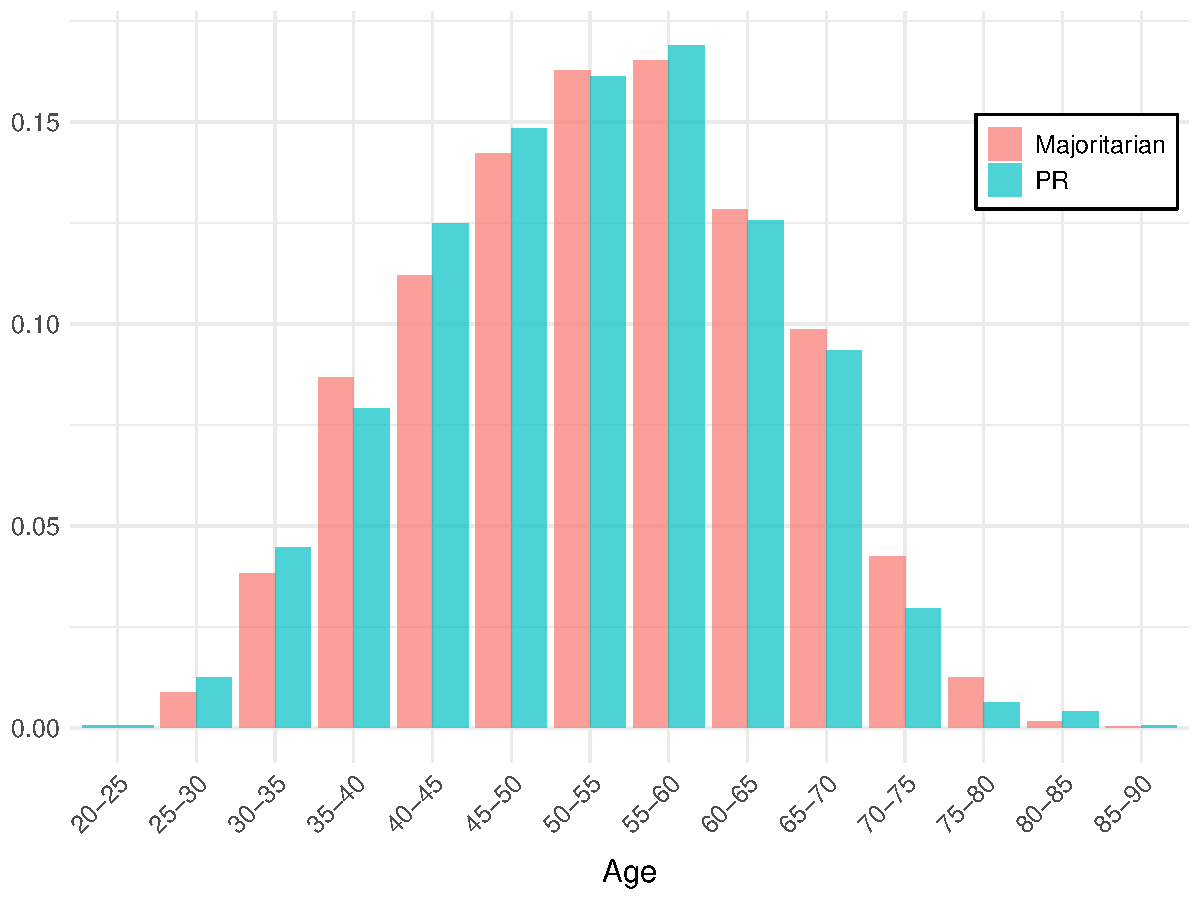
\includegraphics[width = 0.9\textwidth]{../figure/paper/age_smd_vs_pr_winners.pdf}
	\caption{Age Composition of Legislators Elected from the Two Tiers}
	\label{fig:pr_vs_smd}
\end{figure}

The degree of youth descriptive representation in the legislature is largely contingent upon two factors: the frequency of new legislators' entry and the age at which these legislators begin their tenure. Dual listing creates an incentive for political parties to prioritize incumbent and senior candidates by providing them with insurance. This practice may consequently hinder the entry of new legislators, particularly younger ones, into the proportional representation districts, thereby limiting generational renewal within the legislative body.

What would have happened if parties had not been allowed to take that option? To consider the causal effect of allowing dual listing on youth representation in parliament, one needs to identify whom and how parties would have been nominated in the absence of dual listing. This task is daunting: since we are interested in the effect of an electoral rule, we need to specify the point of divergence, i.e., a point where dual listing had become prohibited, but there are too many possibilities. For example, it could have been at the point of the 1994 electoral reform or later than that. In addition, even if we could specify the starting point of the counterfactual scenario, it would be all the more difficult to consider parties' nomination strategies absent dual listing. Parties can adapt to the external environment: since the 1994 reform, parties in Japan have adapted their strategies to the new electoral rules. It would not be clear what kind of candidates parties had nominated if dual listing had not been allowed. 

However, it would not be unreasonable to partially extrapolate the identities of counterfactual nominees from observed data. Specifically, I consider the age of candidates who would have been nominated absent the dual listing option and claim that young citizens would have been better represented in this situation. Recall that dual listing forces parties into a tradeoff between giving second chances to existing candidates and nominating new candidates. Without dual listing, this dilemma disappears, and parties would replace existing SMD candidates with new candidates whose age would be lower than the average candidate or those they replace. Figure \ref{fig:ageFirstRun} compares the average age of candidates (solid lines) with that of candidates running for the first time (dashed lines) across the two tiers (red) and focusing on the PR tier (blue). In each election, new candidates are about three years younger than the average. Narrowing down to the PR tier, new candidates are about three to five years younger than the average. The same patterns apply when comparing the age of winners to that of those elected for the first time (Figure \ref{fig:ageFirstWin}). 

\begin{figure}[!htbp]
	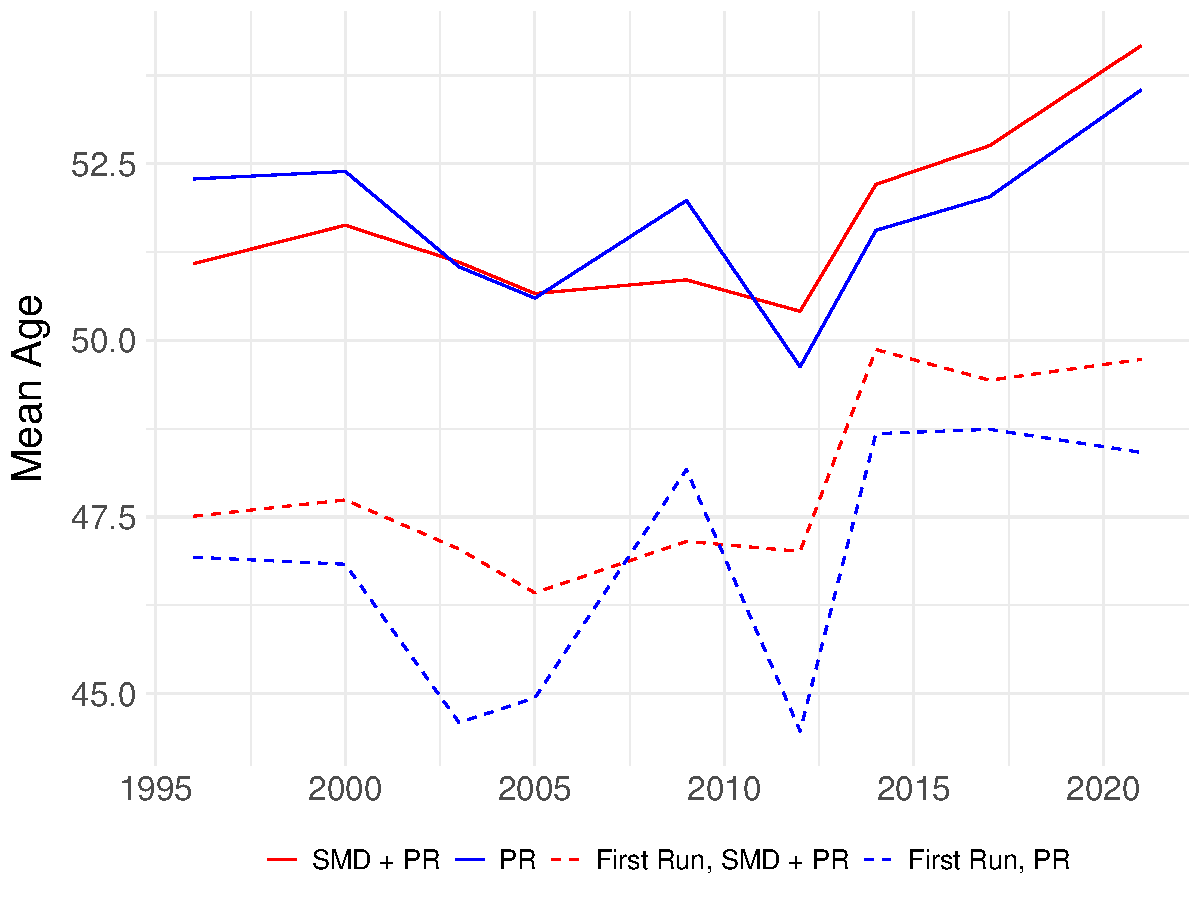
\includegraphics[width = 0.9\textwidth]{../figure/paper/age_first_run.pdf}
	\caption{Age Comparison: Average vs. New Candidates}
	\label{fig:ageFirstRun}
\end{figure}

Since rookie candidates and new MPs are younger than the average, one could reasonably expect that candidates who would have run in the absence of dual listing would have contributed to mitigating youth underrepresentation in parliament. Of course, parties may have adopted a different nomination strategy under this hypothetical scenario. For example, they might have nominated some of the senior candidates and incumbents in the PR tier, where they can expect certain seat gains, and other candidates in the majoritarian tier. However, even in such cases, youth underrepresentation would have been mitigated across the two layers of the system. 

\section{Conclusion}

This paper analyzes the candidate nomination strategies of political parties under the PR system embedded within a mixed electoral system. Using the case of Japan’s House of Representatives elections, it discusses how parties nominate candidates in the proportional representation district when there may be interactions between majoritarian and proportional tiers.

There are two main findings of this paper: First, as commonly seen under a pure PR system, parties give more advantageous rankings to seniors and incumbents. Many parties do not merely aim to maximize votes; they are also mindful of post-election goals such as policy implementation, legislative activities, and the maintenance of party organization. To achieve these, it is not just about increasing the number of legislators sent to parliament but also about continuously electing experienced politicians who have greater resources. Given the monotonic relationship between a candidate’s list rank and their likelihood of election under closed-list PR, parties strategically place incumbents at the top of the list. This nomination strategy is universally observed regardless of the party’s size or the timing of the election.

Moreover, parties use the dual listing mechanism, which allows the same candidate to run in both majoritarian and proportional tiers, to further increase the election chances of senior and incumbent candidates. Whether or not this mechanism is used varies by party: in this paper's analysis, majority-seeking parties such as the LDP and the DPJ / CDP used dual listing to favor senior and incumbent candidates by giving them higher rankings. In contrast, smaller parties like the JCP did not necessarily favor these candidates through dual listing. However, even in times of candidate turnover, such as during the LDP's internal conflicts prior to the 2005 election or after the regime change in the 2009 election, the aforementioned mechanism was still employed.

The findings of this paper have implications for important topics in comparative politics, such as legislative turnover and minority representation. While parties have a default incentive to favor existing candidates, dual listing further amplifies this incentive. Given that the number of seats a party can realistically secure and the number of candidates it can field are both limited, parties must develop their nomination strategies within these constraints. Dual listing, which intensifies the motivation to favor senior and incumbent candidates, is likely to reduce the frequency of turnover.

Additionally, without appropriate institutional design, mixed-member systems may undermine the institutional advantages of proportional representation. Whether minority representation advances under PR systems depends primarily on how many minority candidates are nominated by the parties. Party behavior is shaped by institutional expectations, and in this sense, the dual listing system acts as a barrier to the advancement of minority representation. Focusing on the perspective of minority representation, it can be said that Japan's mixed-member system functions similarly to a majoritarian system.

Future research should analyze candidate nomination patterns in other countries using mixed-member systems. It would be desirable to examine how different types of mixed-member systems generate differences in nomination strategies. For example, the case of Japan analyzed in this paper is a type of MMM system where vote-seat conversion in majoritarian and proportional tiers is independent. However, it would be interesting to explore what nomination strategies are adopted under MMP systems, where seat allocation is determined based on the results of the PR tier. Similarly, it would be intriguing to investigate what outcomes emerge in mixed-member systems that use open-list proportional representation, unlike the closed-list PR system in Japan. In an open-list PR system, the ability to attract personal votes becomes crucial \citep{nemoto_localism_2013, shugart_looking_2005}. In such situations, the incentive for parties to diversify their candidate portfolio is likely to increase, intensifying the trade-off with the incentive to favor existing candidates. Furthermore, it is important to examine whether the patterns observed in this analysis are also found in other countries, such as Germany and New Zealand, where dual listing is available.

\newpage

\bibliography{../Reference.bib}
\bibliographystyle{apalike}

\newpage

\appendix

\setcounter{table}{0}
\setcounter{figure}{0}
\renewcommand{\thetable}{A\arabic{table}}
\renewcommand{\thefigure}{A\arabic{figure}}

\section{Summary Statistics}

\subsection{Candidate-Level Summary}

\begin{table}[!htbp] \centering \renewcommand*{\arraystretch}{1.1}\caption{Summary Statistics}\resizebox{\textwidth}{!}{
\begin{threeparttable}
\begin{tabular}{l|cccccccc}
\toprule
Variable & N & Mean / \% & Std. Dev. & Min & \% 25 & \% 50 & \% 75 & Max \\ 
\midrule
Gender & 6935 &  &  &  &  &  &  &  \\ 
... Female & 881 & 12.7\% &  &  &  &  &  &  \\ 
... Male & 6054 & 87.3\% &  &  &  &  &  &  \\ 
N of wins before & 6935 & 1.776 & 2.487 & 0 & 0 & 1 & 3 & 19 \\ 
Incumbency & 6935 &  &  &  &  &  &  &  \\ 
... Incumbent & 3129 & 45.1\% &  &  &  &  &  &  \\ 
... Non-Incumbent & 3806 & 54.9\% &  &  &  &  &  &  \\ 
List Rank & 6935 & 4.317 & 6.976 & 1 & 1 & 2 & 4 & 52\\ 
Dual Listing & 6935 &  &  &  &  &  &  &  \\ 
... Yes & 5292 & 76.3\% &  &  &  &  &  &  \\ 
... No & 1643 & 23.7\% &  &  &  &  &  &  \\ 
\bottomrule
\end{tabular}
\begin{tablenotes}[flushleft]
  \scriptsize{
    \item Candidate-level summary statistics. 
    \item \textit{Data source}: \citet{reedsmith2018} 
  }
\end{tablenotes}
\end{threeparttable}
}
\label{tab:stats}
\end{table}



\newpage

\subsection{Magnitudes of PR Blocks, 1996 - 2017}

% created manually
\begin{table}[!htbp]
\begin{threeparttable}
\begin{tabular}{lccccccccc}
\toprule
Bloc & 1996 & 2000 & 2003 & 2005 & 2009 & 2012 & 2014 & 2017 & 2021 \\
\midrule
Hokkaido & 9 & 8 & 8 & 8 & 8 & 8 & 8 & 8 & 8 \\
Tohoku & 16 & 14 & 14 & 14 & 14 & 14 & 14 & 13 & 13 \\
Kita-kanto & 21 & 20 & 20 & 20 & 20 & 20 & 20 & 19 & 19 \\
Tokyo & 19 & 17 & 17 & 17 & 17 & 17 & 17 & 17 & 17 \\
Minami-kanto & 23 & 21 & 22 & 22 & 22 & 22 & 22 & 22 & 22 \\
Hokuriku Shinetsu & 13 & 11 & 11 & 11 & 11 & 11 & 11 & 11 & 11 \\
Tokai & 23 & 21 & 21 & 21 & 21 & 21 & 21 & 21 & 21 \\
Kinki & 33 & 30 & 30 & 30 & 29 & 29 & 29 & 28 & 28 \\
Chugoku & 13 & 11 & 11 & 11 & 11 & 11 & 11 & 11 & 11 \\
Shikoku & 7 & 6 & 6 & 6 & 6 & 6 & 6 & 6 & 6 \\
Kyushu & 23 & 21 & 21 & 21 & 21 & 21 & 21 & 20 & 20 \\
\bottomrule
\end{tabular}
\begin{tablenotes}[flushleft]
  \scriptsize{
    \item Magnitudes of each PR regional district for elections 1996 - 2021. 
    \item \textit{Data source}: \citet{reedReedSmithJapaneseHouse2017, ministryofinternalaffairsandcommunicationsElectionSenkyo2024}
  }
\end{tablenotes}
\end{threeparttable}
\caption{Magnitudes of PR Blocks}
\label{tab:distM}
\end{table}

\newpage

\subsection{Distribution of List Rank}

\begin{figure}[!htbp]
	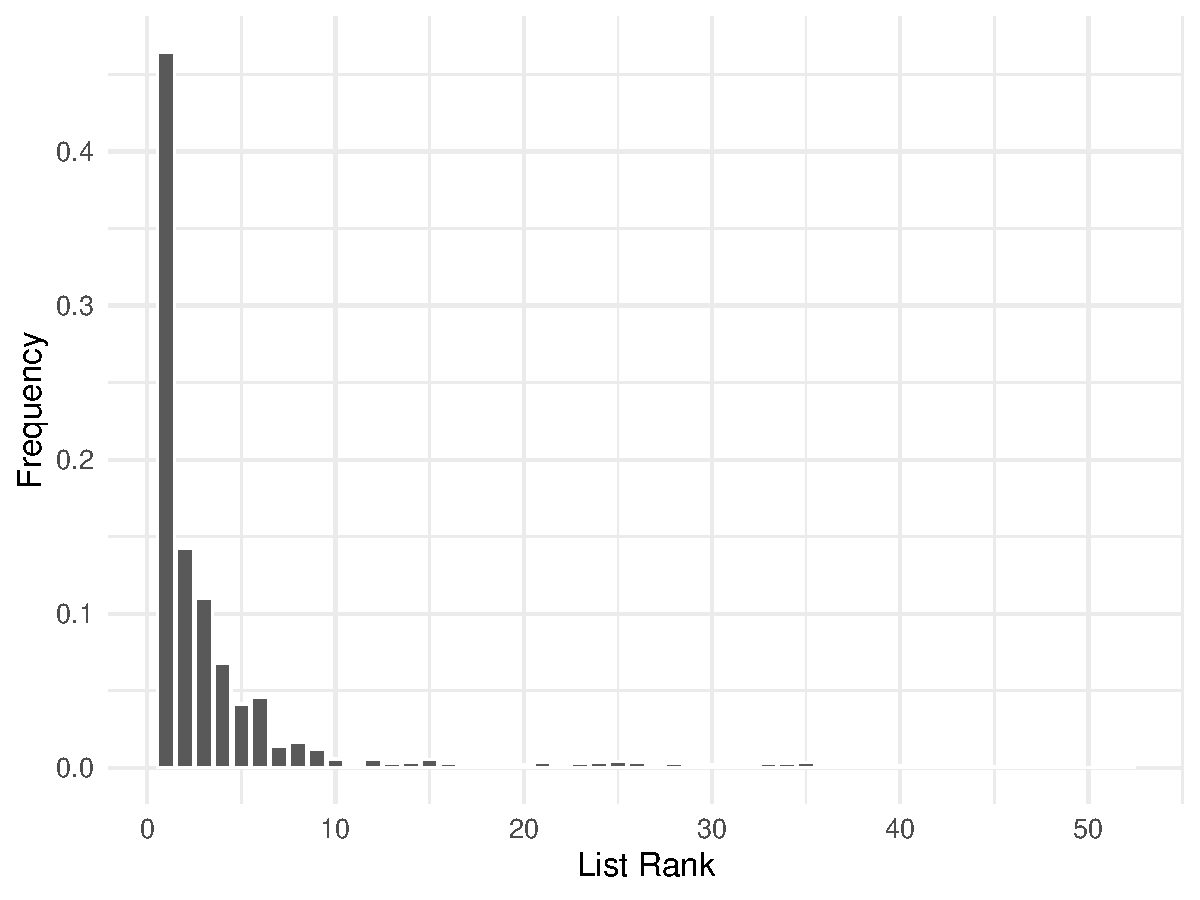
\includegraphics[width = 0.9\textwidth]{../figure/paper/pr_rank_distribution.pdf}
	\caption{Distribution of List Rank}
	\label{fig:distRank}
\end{figure}

\newpage

\subsection{Age of Winners}

\begin{figure}[!htbp]
	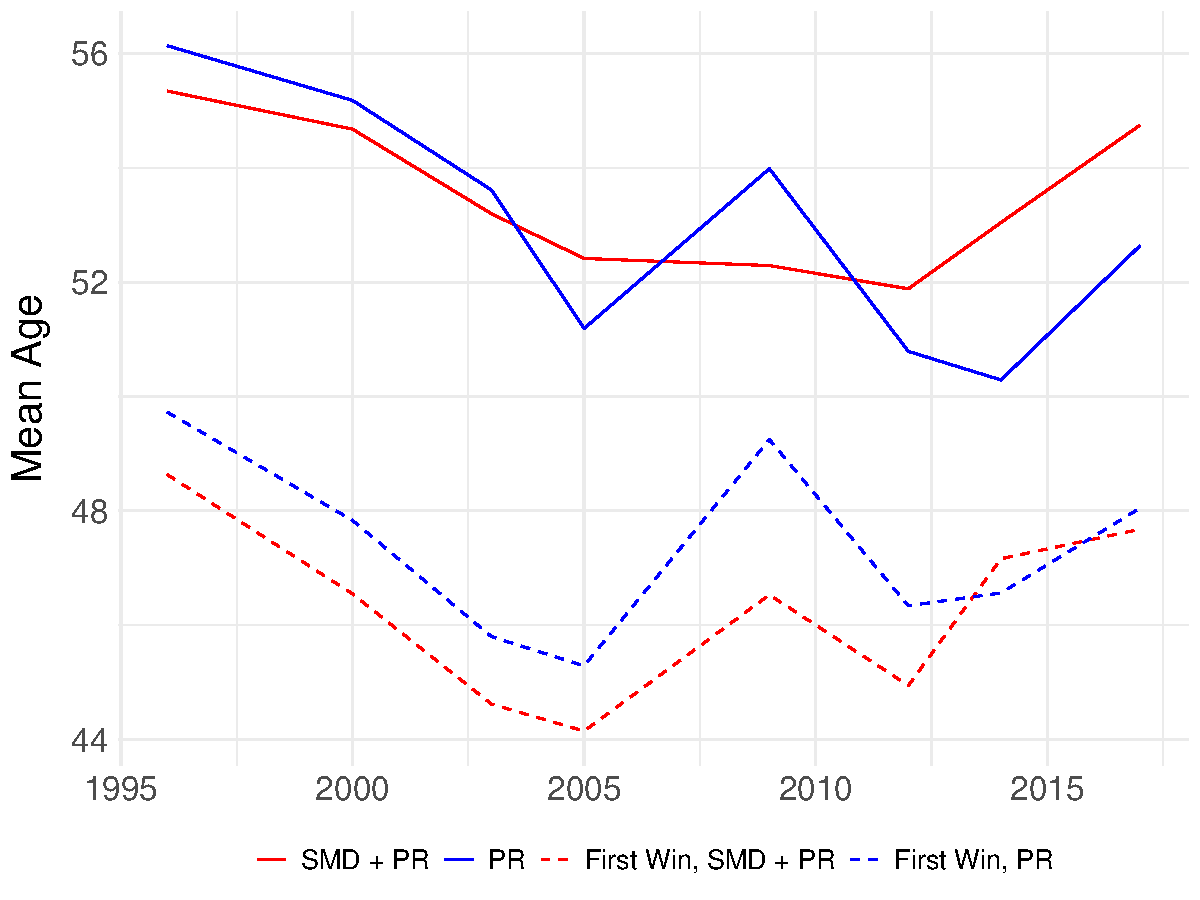
\includegraphics[width = 0.9\textwidth]{../figure/paper/age_first_win.pdf}
	\caption{Age Comparison: Average vs. New Legislators}
	\label{fig:ageFirstWin}
\end{figure}	

\newpage

\section{Additional Analyses}

\setcounter{table}{0}
\setcounter{figure}{0}
\renewcommand{\thetable}{B\arabic{table}}
\renewcommand{\thefigure}{B\arabic{figure}}

\subsection{Regression Analysis for DPJ / CDP Candidates}


\begin{table}[!bth]
\begin{center}
\begin{threeparttable}
\begin{tabular}{l D{.}{.}{4.5} D{.}{.}{4.5} D{.}{.}{5.5} D{.}{.}{5.5} D{.}{.}{5.5}}
\toprule
 & \multicolumn{2}{c}{Dual Listing} & \multicolumn{3}{c}{List Rank} \\
\cmidrule(lr){2-3} \cmidrule(lr){4-6}
 & \multicolumn{1}{c}{H1} & \multicolumn{1}{c}{H2} & \multicolumn{1}{c}{H3} & \multicolumn{1}{c}{H4} & \multicolumn{1}{c}{H5} \\
\midrule
Total Wins      & 0.35^{***}              &                         & -0.14^{***}             &                         &                         \\
                & (0.07)                  &                         & (0.01)                  &                         &                         \\
Incumbency      &                         & 1.25^{***}              &                         & -0.74^{***}             &                         \\
                &                         & (0.24)                  &                         & (0.06)                  &                         \\
Dual Listing    &                         &                         &                         &                         & -2.53^{***}             \\
                &                         &                         &                         &                         & (0.05)                  \\
Female          & -0.04                   & -0.11                   & -0.00                   & -0.02                   & -0.01                   \\
                & (0.24)                  & (0.24)                  & (0.08)                  & (0.08)                  & (0.06)                  \\
Block Magnitude & 0.04^{**}               & 0.04^{**}               & 0.01^{**}               & 0.01^{***}              & 0.02^{***}              \\
                & (0.01)                  & (0.01)                  & (0.00)                  & (0.00)                  & (0.00)                  \\
\midrule
Year FE         & \multicolumn{1}{c}{Yes} & \multicolumn{1}{c}{Yes} & \multicolumn{1}{c}{Yes} & \multicolumn{1}{c}{Yes} & \multicolumn{1}{c}{Yes} \\
Party FE        & \multicolumn{1}{c}{Yes} & \multicolumn{1}{c}{Yes} & \multicolumn{1}{c}{Yes} & \multicolumn{1}{c}{Yes} & \multicolumn{1}{c}{Yes} \\
AIC             & 949.35                  & 951.02                  & 8026.35                 & 7974.18                 & 6423.06                 \\
BIC             & 1010.13                 & 1011.79                 & 8092.65                 & 8040.48                 & 6489.36                 \\
Log Likelihood  & -463.68                 & -464.51                 & -4001.17                & -3975.09                & -3199.53                \\
Deviance        & 927.35                  & 929.02                  & 1608.56                 & 1589.41                 & 1033.39                 \\
Num. obs.       & 1854                    & 1854                    & 1854                    & 1854                    & 1854                    \\
\bottomrule
\end{tabular}
\begin{tablenotes}[flushleft]
\scriptsize{\item $^{***}p<0.001$; $^{**}p<0.01$; $^{*}p<0.05$. Standard errors in parentheses.
\item Dependent variable: candidate $i$'s list rank (H1-2) and dual nomination status (H3-5).
\item Estimated models: logit (H1-2) and negative binomial (H3-5).}
\end{tablenotes}
\end{threeparttable}
\caption{Regression Results for DPJ / CDP Candidates}
\label{tab:regDPJCDP}
\end{center}
\end{table}


\newpage

\subsection{Regression Analysis for Komeito Candidates}


\begin{table}
\begin{center}
\begin{tabular}{l c c c c c c c c c c}
\hline
 & \multicolumn{4}{c}{List Rank} & \multicolumn{3}{c}{Dual Listing} & \multicolumn{3}{c}{Dual Listing (Tie)} \\
\cline{2-5} \cline{6-8} \cline{9-11}
 & Model 1 & Model 2 & Model 3 & Model 4 & Model 5 & Model 6 & Model 7 & Model 8 & Model 9 & Model 10 \\
\hline
Total Wins       & $-0.21^{***}$ &               &           & $-0.12^{***}$ & $0.32$   &          & $0.12$   & $0.34$   &          & $0.38$   \\
                 & $(0.02)$      &               &           & $(0.03)$      & $(0.19)$ &          & $(0.27)$ & $(0.24)$ &          & $(0.34)$ \\
Incumbency       &               & $-0.79^{***}$ &           & $-0.46^{***}$ &          & $1.50$   & $1.21$   &          & $1.17$   & $0.35$   \\
                 &               & $(0.07)$      &           & $(0.12)$      &          & $(0.88)$ & $(1.15)$ &          & $(1.25)$ & $(1.70)$ \\
Dual Listing     &               &               & $-0.26$   & $0.20$        &          &          &          &          &          &          \\
                 &               &               & $(0.23)$  & $(0.30)$      &          &          &          &          &          &          \\
Tie              &               &               &           & $-1.63$       &          &          &          &          &          &          \\
                 &               &               &           & $(1.96)$      &          &          &          &          &          &          \\
Female           &               &               &           & $-0.13$       &          &          & $-0.49$  &          &          & $1.06$   \\
                 &               &               &           & $(0.10)$      &          &          & $(1.19)$ &          &          & $(1.45)$ \\
Block Magnitude  &               &               &           & $0.04^{***}$  &          &          & $-0.06$  &          &          & $-0.05$  \\
                 &               &               &           & $(0.01)$      &          &          & $(0.06)$ &          &          & $(0.10)$ \\
Total Wins x Tie &               &               &           & $0.64$        &          &          &          &          &          &          \\
                 &               &               &           & $(0.71)$      &          &          &          &          &          &          \\
\hline
Year FE          & Yes           & Yes           & Yes       & Yes           & Yes      & Yes      & Yes      & Yes      & Yes      & Yes      \\
Party FE         & No            & No            & No        & No            & No       & No       & No       & No       & No       & No       \\
AIC              & $18.00$       & $1134.87$     & $1264.37$ & $1042.07$     & $57.30$  & $56.69$  & $61.28$  & $38.40$  & $39.19$  & $43.55$  \\
BIC              & $52.05$       & $1168.92$     & $1298.42$ & $1098.83$     & $87.57$  & $86.96$  & $102.91$ & $68.67$  & $69.46$  & $85.18$  \\
Log Likelihood   & $0.00$        & $-558.43$     & $-623.18$ & $-506.04$     & $-20.65$ & $-20.35$ & $-19.64$ & $-11.20$ & $-11.59$ & $-10.78$ \\
Deviance         & $180.36$      & $195.93$      & $309.02$  & $91.14$       & $41.30$  & $40.69$  & $39.28$  & $22.40$  & $23.19$  & $21.55$  \\
Num. obs.        & $325$         & $325$         & $325$     & $325$         & $325$    & $325$    & $325$    & $325$    & $325$    & $325$    \\
\hline
\multicolumn{11}{l}{\scriptsize{\item $^{***}p<0.001$; $^{**}p<0.01$; $^{*}p<0.05$. Standard errors in parentheses.
\item Dependent variable: candidate $i$'s list rank (columns 1-4) dual listing status (columns 5-7), and whether the candidate has a tie on the list (columns 8-10).
\item Estimated models: negatige binomial (columns 1-4) and logit (columns 5-10).}}
\end{tabular}
\caption{Regression Results for Komeito Candidates}
\label{tab:komeito}
\end{center}
\end{table}


\end{document}































